\newcommand{\coursemodule}{Module 08}
% ════════════════════════════════════════════════════════════════════════════
% Pixels, Frames & Transformers: shared Beamer preamble (WUR style)
% Adapted from the preamble of Bags, Vectors & Transformers.
%
% Use in a module deck (from <part>/<module>/slides/):
%   \newcommand{\coursemodule}{Module 01}
%   % ════════════════════════════════════════════════════════════════════════════
% Pixels, Frames & Transformers: shared Beamer preamble (WUR style)
% Adapted from the preamble of Bags, Vectors & Transformers.
%
% Use in a module deck (from <part>/<module>/slides/):
%   \newcommand{\coursemodule}{Module 01}
%   % ════════════════════════════════════════════════════════════════════════════
% Pixels, Frames & Transformers: shared Beamer preamble (WUR style)
% Adapted from the preamble of Bags, Vectors & Transformers.
%
% Use in a module deck (from <part>/<module>/slides/):
%   \newcommand{\coursemodule}{Module 01}
%   \input{../../../shared/preamble.tex}
%   \begin{document}
%   \moduletitle{Images as Data}
%   ...
% Compile with: latexmk -pdf <deck>.tex
% ════════════════════════════════════════════════════════════════════════════

\documentclass[aspectratio=169]{beamer}

% ── Packages ────────────────────────────────────────────────────────────────
\usepackage[T1]{fontenc}
\usepackage[utf8]{inputenc}
\usepackage{lmodern}
\usepackage{microtype}
\usepackage{xcolor}
\usepackage{tikz}
\usetikzlibrary{arrows.meta, positioning, calc, shapes.geometric, decorations.pathreplacing, matrix, fit}
\usepackage{booktabs}
\usepackage{fontawesome5}
\usepackage{array}
\usepackage[most]{tcolorbox}

\providecommand{\coursemodule}{}

% ── WUR color palette ───────────────────────────────────────────────────────
\definecolor{wurgreen}{HTML}{34B233}
\definecolor{darkgreen}{HTML}{1F6B1E}
\definecolor{lightgreen}{HTML}{E8F7E8}
\definecolor{darknavy}{HTML}{1A1A2E}
\definecolor{midgray}{HTML}{6B7280}
\definecolor{lightgray}{HTML}{F3F4F6}
\definecolor{bodytext}{HTML}{1F2937}
\definecolor{codegreen}{HTML}{9AE6B4}
\definecolor{warnred}{HTML}{FEE2E2}
\definecolor{warnborder}{HTML}{EF4444}

% ── Beamer theme ────────────────────────────────────────────────────────────
\usetheme{default}
\usecolortheme{default}
\usefonttheme{professionalfonts}
\setbeamertemplate{navigation symbols}{}
\setbeamertemplate{itemize items}{\textcolor{wurgreen}{\textbullet}}
\setbeamertemplate{itemize subitem}{\textcolor{midgray}{--}}
\setbeamertemplate{enumerate items}{\textcolor{wurgreen}{\textbf{\insertenumlabel.}}}
\setbeamercolor{frametitle}{fg=white, bg=darknavy}
\setbeamertemplate{frametitle}{%
  \begin{beamercolorbox}[wd=\paperwidth, ht=1.1cm, dp=0.2cm, leftskip=0.6cm]{frametitle}
    \usebeamerfont{frametitle}\insertframetitle
  \end{beamercolorbox}%
}
\setbeamerfont{frametitle}{size=\large, series=\bfseries}
\setbeamercolor{background canvas}{bg=white}
\setbeamercolor{normal text}{fg=bodytext}
\setbeamerfont{normal text}{size=\small}
\setbeamertemplate{footline}{%
  \begin{beamercolorbox}[wd=\paperwidth, ht=0.4cm, dp=0.15cm]{footline}%
    \hspace{0.5cm}%
    \textcolor{midgray}{\tiny Pixels, Frames \& Transformers · \coursemodule\ · Wageningen University \& Research}%
    \hfill%
    \textcolor{midgray}{\tiny \insertframenumber}%
    \hspace{0.4cm}%
  \end{beamercolorbox}%
}

% ── Boxes ───────────────────────────────────────────────────────────────────
\tcbset{wurbase/.style={arc=3pt, boxrule=0.6pt, left=7pt, right=7pt, top=5pt, bottom=5pt,
                        fontupper=\small, before skip=4pt, after skip=4pt}}
\newtcolorbox{greenbox}[1][]{wurbase, colback=lightgreen, colframe=wurgreen, #1}
\newtcolorbox{graybox}[1][]{wurbase, colback=lightgray, colframe=lightgray, #1}
\newtcolorbox{navybox}[1][]{wurbase, colback=darknavy, colframe=darknavy, colupper=white, #1}
\newtcolorbox{warnbox}[1][]{wurbase, colback=warnred, colframe=warnborder, #1}
\newtcolorbox{codebox}[1][]{wurbase, colback=darknavy, colframe=darknavy, colupper=white,
                            fontupper=\ttfamily\scriptsize, left=6pt, top=4pt, bottom=4pt, #1}

% ── Title slide ─────────────────────────────────────────────────────────────
\newcommand{\moduletitle}[1]{%
{
\setbeamertemplate{footline}{}
\begin{frame}[plain]
  \begin{tikzpicture}[remember picture, overlay]
    \fill[darknavy] (current page.south west) rectangle (current page.north east);
    \fill[wurgreen] (current page.south west) rectangle ([xshift=0.45cm]current page.north west);
    \node[anchor=west, text=white, font=\huge\bfseries, text width=13cm]
      at ([xshift=1.1cm, yshift=1.2cm]current page.west) {Pixels, Frames \& Transformers};
    \node[anchor=west, text=wurgreen, font=\large, text width=13cm]
      at ([xshift=1.1cm, yshift=0.05cm]current page.west) {#1 · \coursemodule};
    \node[anchor=west, text=midgray, font=\small, text width=12cm]
      at ([xshift=1.1cm, yshift=-1.5cm]current page.west)
      {Denise J. Roth, PhD Candidate\\
       Strategic Communication Group · Wageningen University \& Research};
  \end{tikzpicture}
\end{frame}
}}

% ── Small helpers ───────────────────────────────────────────────────────────
\newcommand{\keyterm}[1]{\textbf{\textcolor{darkgreen}{#1}}}
\newcommand{\muted}[1]{\textcolor{midgray}{#1}}
\newcommand{\credit}[1]{{\tiny\textcolor{midgray}{#1}}}
\newcommand{\notebookslide}[1]{%
\begin{frame}{In the Notebook}
\vspace{0.1cm}
#1
\end{frame}}
\newcommand{\nbitem}[2]{\item[\textcolor{wurgreen}{#1}] #2}

%   \begin{document}
%   \moduletitle{Images as Data}
%   ...
% Compile with: latexmk -pdf <deck>.tex
% ════════════════════════════════════════════════════════════════════════════

\documentclass[aspectratio=169]{beamer}

% ── Packages ────────────────────────────────────────────────────────────────
\usepackage[T1]{fontenc}
\usepackage[utf8]{inputenc}
\usepackage{lmodern}
\usepackage{microtype}
\usepackage{xcolor}
\usepackage{tikz}
\usetikzlibrary{arrows.meta, positioning, calc, shapes.geometric, decorations.pathreplacing, matrix, fit}
\usepackage{booktabs}
\usepackage{fontawesome5}
\usepackage{array}
\usepackage[most]{tcolorbox}

\providecommand{\coursemodule}{}

% ── WUR color palette ───────────────────────────────────────────────────────
\definecolor{wurgreen}{HTML}{34B233}
\definecolor{darkgreen}{HTML}{1F6B1E}
\definecolor{lightgreen}{HTML}{E8F7E8}
\definecolor{darknavy}{HTML}{1A1A2E}
\definecolor{midgray}{HTML}{6B7280}
\definecolor{lightgray}{HTML}{F3F4F6}
\definecolor{bodytext}{HTML}{1F2937}
\definecolor{codegreen}{HTML}{9AE6B4}
\definecolor{warnred}{HTML}{FEE2E2}
\definecolor{warnborder}{HTML}{EF4444}

% ── Beamer theme ────────────────────────────────────────────────────────────
\usetheme{default}
\usecolortheme{default}
\usefonttheme{professionalfonts}
\setbeamertemplate{navigation symbols}{}
\setbeamertemplate{itemize items}{\textcolor{wurgreen}{\textbullet}}
\setbeamertemplate{itemize subitem}{\textcolor{midgray}{--}}
\setbeamertemplate{enumerate items}{\textcolor{wurgreen}{\textbf{\insertenumlabel.}}}
\setbeamercolor{frametitle}{fg=white, bg=darknavy}
\setbeamertemplate{frametitle}{%
  \begin{beamercolorbox}[wd=\paperwidth, ht=1.1cm, dp=0.2cm, leftskip=0.6cm]{frametitle}
    \usebeamerfont{frametitle}\insertframetitle
  \end{beamercolorbox}%
}
\setbeamerfont{frametitle}{size=\large, series=\bfseries}
\setbeamercolor{background canvas}{bg=white}
\setbeamercolor{normal text}{fg=bodytext}
\setbeamerfont{normal text}{size=\small}
\setbeamertemplate{footline}{%
  \begin{beamercolorbox}[wd=\paperwidth, ht=0.4cm, dp=0.15cm]{footline}%
    \hspace{0.5cm}%
    \textcolor{midgray}{\tiny Pixels, Frames \& Transformers · \coursemodule\ · Wageningen University \& Research}%
    \hfill%
    \textcolor{midgray}{\tiny \insertframenumber}%
    \hspace{0.4cm}%
  \end{beamercolorbox}%
}

% ── Boxes ───────────────────────────────────────────────────────────────────
\tcbset{wurbase/.style={arc=3pt, boxrule=0.6pt, left=7pt, right=7pt, top=5pt, bottom=5pt,
                        fontupper=\small, before skip=4pt, after skip=4pt}}
\newtcolorbox{greenbox}[1][]{wurbase, colback=lightgreen, colframe=wurgreen, #1}
\newtcolorbox{graybox}[1][]{wurbase, colback=lightgray, colframe=lightgray, #1}
\newtcolorbox{navybox}[1][]{wurbase, colback=darknavy, colframe=darknavy, colupper=white, #1}
\newtcolorbox{warnbox}[1][]{wurbase, colback=warnred, colframe=warnborder, #1}
\newtcolorbox{codebox}[1][]{wurbase, colback=darknavy, colframe=darknavy, colupper=white,
                            fontupper=\ttfamily\scriptsize, left=6pt, top=4pt, bottom=4pt, #1}

% ── Title slide ─────────────────────────────────────────────────────────────
\newcommand{\moduletitle}[1]{%
{
\setbeamertemplate{footline}{}
\begin{frame}[plain]
  \begin{tikzpicture}[remember picture, overlay]
    \fill[darknavy] (current page.south west) rectangle (current page.north east);
    \fill[wurgreen] (current page.south west) rectangle ([xshift=0.45cm]current page.north west);
    \node[anchor=west, text=white, font=\huge\bfseries, text width=13cm]
      at ([xshift=1.1cm, yshift=1.2cm]current page.west) {Pixels, Frames \& Transformers};
    \node[anchor=west, text=wurgreen, font=\large, text width=13cm]
      at ([xshift=1.1cm, yshift=0.05cm]current page.west) {#1 · \coursemodule};
    \node[anchor=west, text=midgray, font=\small, text width=12cm]
      at ([xshift=1.1cm, yshift=-1.5cm]current page.west)
      {Denise J. Roth, PhD Candidate\\
       Strategic Communication Group · Wageningen University \& Research};
  \end{tikzpicture}
\end{frame}
}}

% ── Small helpers ───────────────────────────────────────────────────────────
\newcommand{\keyterm}[1]{\textbf{\textcolor{darkgreen}{#1}}}
\newcommand{\muted}[1]{\textcolor{midgray}{#1}}
\newcommand{\credit}[1]{{\tiny\textcolor{midgray}{#1}}}
\newcommand{\notebookslide}[1]{%
\begin{frame}{In the Notebook}
\vspace{0.1cm}
#1
\end{frame}}
\newcommand{\nbitem}[2]{\item[\textcolor{wurgreen}{#1}] #2}

%   \begin{document}
%   \moduletitle{Images as Data}
%   ...
% Compile with: latexmk -pdf <deck>.tex
% ════════════════════════════════════════════════════════════════════════════

\documentclass[aspectratio=169]{beamer}

% ── Packages ────────────────────────────────────────────────────────────────
\usepackage[T1]{fontenc}
\usepackage[utf8]{inputenc}
\usepackage{lmodern}
\usepackage{microtype}
\usepackage{xcolor}
\usepackage{tikz}
\usetikzlibrary{arrows.meta, positioning, calc, shapes.geometric, decorations.pathreplacing, matrix, fit}
\usepackage{booktabs}
\usepackage{fontawesome5}
\usepackage{array}
\usepackage[most]{tcolorbox}

\providecommand{\coursemodule}{}

% ── WUR color palette ───────────────────────────────────────────────────────
\definecolor{wurgreen}{HTML}{34B233}
\definecolor{darkgreen}{HTML}{1F6B1E}
\definecolor{lightgreen}{HTML}{E8F7E8}
\definecolor{darknavy}{HTML}{1A1A2E}
\definecolor{midgray}{HTML}{6B7280}
\definecolor{lightgray}{HTML}{F3F4F6}
\definecolor{bodytext}{HTML}{1F2937}
\definecolor{codegreen}{HTML}{9AE6B4}
\definecolor{warnred}{HTML}{FEE2E2}
\definecolor{warnborder}{HTML}{EF4444}

% ── Beamer theme ────────────────────────────────────────────────────────────
\usetheme{default}
\usecolortheme{default}
\usefonttheme{professionalfonts}
\setbeamertemplate{navigation symbols}{}
\setbeamertemplate{itemize items}{\textcolor{wurgreen}{\textbullet}}
\setbeamertemplate{itemize subitem}{\textcolor{midgray}{--}}
\setbeamertemplate{enumerate items}{\textcolor{wurgreen}{\textbf{\insertenumlabel.}}}
\setbeamercolor{frametitle}{fg=white, bg=darknavy}
\setbeamertemplate{frametitle}{%
  \begin{beamercolorbox}[wd=\paperwidth, ht=1.1cm, dp=0.2cm, leftskip=0.6cm]{frametitle}
    \usebeamerfont{frametitle}\insertframetitle
  \end{beamercolorbox}%
}
\setbeamerfont{frametitle}{size=\large, series=\bfseries}
\setbeamercolor{background canvas}{bg=white}
\setbeamercolor{normal text}{fg=bodytext}
\setbeamerfont{normal text}{size=\small}
\setbeamertemplate{footline}{%
  \begin{beamercolorbox}[wd=\paperwidth, ht=0.4cm, dp=0.15cm]{footline}%
    \hspace{0.5cm}%
    \textcolor{midgray}{\tiny Pixels, Frames \& Transformers · \coursemodule\ · Wageningen University \& Research}%
    \hfill%
    \textcolor{midgray}{\tiny \insertframenumber}%
    \hspace{0.4cm}%
  \end{beamercolorbox}%
}

% ── Boxes ───────────────────────────────────────────────────────────────────
\tcbset{wurbase/.style={arc=3pt, boxrule=0.6pt, left=7pt, right=7pt, top=5pt, bottom=5pt,
                        fontupper=\small, before skip=4pt, after skip=4pt}}
\newtcolorbox{greenbox}[1][]{wurbase, colback=lightgreen, colframe=wurgreen, #1}
\newtcolorbox{graybox}[1][]{wurbase, colback=lightgray, colframe=lightgray, #1}
\newtcolorbox{navybox}[1][]{wurbase, colback=darknavy, colframe=darknavy, colupper=white, #1}
\newtcolorbox{warnbox}[1][]{wurbase, colback=warnred, colframe=warnborder, #1}
\newtcolorbox{codebox}[1][]{wurbase, colback=darknavy, colframe=darknavy, colupper=white,
                            fontupper=\ttfamily\scriptsize, left=6pt, top=4pt, bottom=4pt, #1}

% ── Title slide ─────────────────────────────────────────────────────────────
\newcommand{\moduletitle}[1]{%
{
\setbeamertemplate{footline}{}
\begin{frame}[plain]
  \begin{tikzpicture}[remember picture, overlay]
    \fill[darknavy] (current page.south west) rectangle (current page.north east);
    \fill[wurgreen] (current page.south west) rectangle ([xshift=0.45cm]current page.north west);
    \node[anchor=west, text=white, font=\huge\bfseries, text width=13cm]
      at ([xshift=1.1cm, yshift=1.2cm]current page.west) {Pixels, Frames \& Transformers};
    \node[anchor=west, text=wurgreen, font=\large, text width=13cm]
      at ([xshift=1.1cm, yshift=0.05cm]current page.west) {#1 · \coursemodule};
    \node[anchor=west, text=midgray, font=\small, text width=12cm]
      at ([xshift=1.1cm, yshift=-1.5cm]current page.west)
      {Denise J. Roth, PhD Candidate\\
       Strategic Communication Group · Wageningen University \& Research};
  \end{tikzpicture}
\end{frame}
}}

% ── Small helpers ───────────────────────────────────────────────────────────
\newcommand{\keyterm}[1]{\textbf{\textcolor{darkgreen}{#1}}}
\newcommand{\muted}[1]{\textcolor{midgray}{#1}}
\newcommand{\credit}[1]{{\tiny\textcolor{midgray}{#1}}}
\newcommand{\notebookslide}[1]{%
\begin{frame}{In the Notebook}
\vspace{0.1cm}
#1
\end{frame}}
\newcommand{\nbitem}[2]{\item[\textcolor{wurgreen}{#1}] #2}


\begin{document}

\moduletitle{Vision Transformers}

% ─────────────────────────────────────────────────────────────────────────────
\begin{frame}{An Image Is Worth 16 $\times$ 16 Words}
\begin{columns}[T]
\begin{column}{0.52\textwidth}
In 2020, Dosovitskiy and colleagues took the transformer from language models, changed almost
nothing, and fed it images cut into small squares.

\vspace{0.2cm}
\begin{itemize}
\item Each 16 $\times$ 16 pixel \keyterm{patch} becomes a token, like a word
\item The same self-attention layers as BERT
\item Trained on enough images, it matched the best CNNs
\end{itemize}
\end{column}
\begin{column}{0.44\textwidth}
\begin{greenbox}
\textbf{Why it matters for this course}\\
ViTs are inside almost everything that follows: CLIP (module 09), vision-language models
(10, 11), open-vocabulary detectors and SAM (12), and the video models of Part 4.
\end{greenbox}
\muted{\footnotesize Dosovitskiy et al.\ (2021), ICLR.}
\end{column}
\end{columns}
\end{frame}

% ─────────────────────────────────────────────────────────────────────────────
\begin{frame}{Patches as Tokens}
\centering
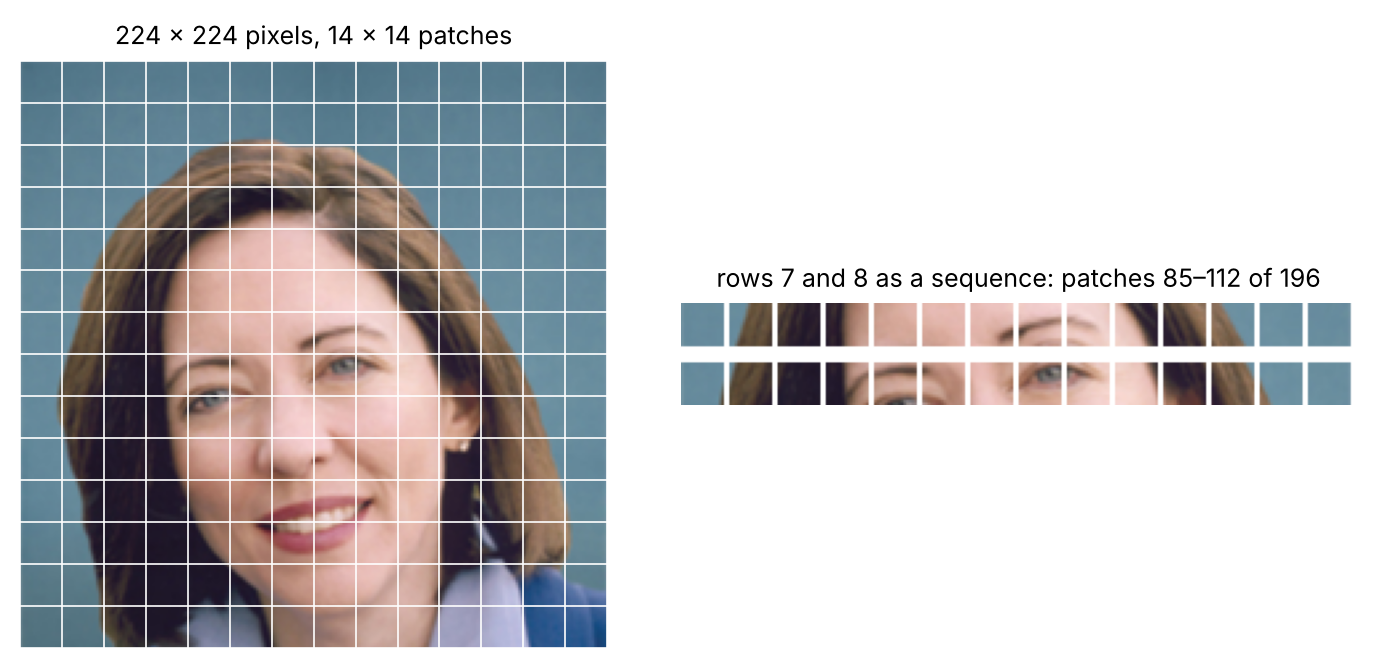
\includegraphics[width=0.74\textwidth]{figures/patches.png}

\vspace{0.05cm}
\raggedright
{\small Each patch is 16 $\times$ 16 $\times$ 3 = 768 numbers. One linear layer turns it into the patch's
token embedding; a learned \keyterm{position embedding} is added so the model knows where the
patch was. A \keyterm{class token} at the front collects a summary of the whole image.}

\vspace{0.1cm}
\credit{Official portrait of Sen.\ Maria Cantwell, public domain, via unitedstates/images.}
\end{frame}

% ─────────────────────────────────────────────────────────────────────────────
\begin{frame}{BERT and ViT, Side by Side}
\vspace{0.1cm}
\centering
{\small
\begin{tabular}{@{}p{3.0cm}p{3.9cm}p{3.9cm}@{}}
\toprule
 & \textbf{BERT} (text) & \textbf{ViT} (images) \\
\midrule
input unit & a word piece & a 16 $\times$ 16 pixel patch \\
token embedding & looked up in a vocabulary & computed from the pixels \\
order & position embeddings & position embeddings (2D layout learned) \\
summary token & \texttt{[CLS]} & class token \\
layers & self-attention + MLP & the same \\
pre-training & guess masked words & image labels, or self-supervised \\
the usual embedding & \texttt{[CLS]} or mean of tokens & class token \\
\bottomrule
\end{tabular}}

\vspace{0.3cm}
\raggedright
\muted{If you know the BERT deck of Bags, Vectors \& Transformers, you already know most of a ViT.
The new part is how the tokens are made.}
\end{frame}

% ─────────────────────────────────────────────────────────────────────────────
\begin{frame}{Every Patch Sees Every Patch}
\begin{columns}[T]
\begin{column}{0.5\textwidth}
\begin{itemize}
\item A CNN filter sees a small neighborhood; opposite corners of the image only meet after many
      layers
\item In a ViT, \keyterm{self-attention} lets each token take information from every other token,
      from the first layer on
\item The price: attention compares all pairs, so cost grows with the \textbf{square} of the
      number of tokens
\end{itemize}
\end{column}
\begin{column}{0.46\textwidth}
{\footnotesize
\begin{tabular}{@{}lrr@{}}
\toprule
image, patch & tokens & attention \\
\midrule
224, 32 \muted{(CLIP B/32)} & 50 & 2,500 \\
224, 16 & 197 & 38,809 \\
384, 16 & 577 & 332,929 \\
518, 14 \muted{(DINOv2)} & 1,370 & 1,876,900 \\
\bottomrule
\end{tabular}}

\vspace{0.2cm}
\muted{\footnotesize Double the image size, and attention costs about 16 times as much. Small
details, like text on a sign, can vanish inside a large patch.}
\end{column}
\end{columns}
\end{frame}

% ─────────────────────────────────────────────────────────────────────────────
\begin{frame}{Why ViTs Need More Data}
\begin{columns}[T]
\begin{column}{0.5\textwidth}
A CNN has assumptions built in: nearby pixels belong together, and a pattern means the same thing
anywhere in the image. A ViT has to \textbf{learn} these from data.

\vspace{0.2cm}
\begin{itemize}
\item Trained on ImageNet's 1.3 million images alone, the original ViT did worse than ResNets
\item Pre-trained on 14 million images (ImageNet-21k) it caught up, and on 300 million it did better
\end{itemize}
\end{column}
\begin{column}{0.46\textwidth}
\begin{graybox}
\textbf{What this means for you}\\
Never train a ViT from scratch on social science data. Start from a pre-trained one: as a frozen
embedding with a linear probe, or fine-tuned with a small learning rate.
\end{graybox}
\muted{\footnotesize Later work (such as DeiT, Touvron et al., 2021) made ViTs trainable on
ImageNet alone with heavy augmentation, but the advice stands.}
\end{column}
\end{columns}
\end{frame}

% ─────────────────────────────────────────────────────────────────────────────
\begin{frame}{Pre-Training Without Labels}
\begin{columns}[T]
\begin{column}{0.48\textwidth}
\begin{greenbox}[height=3.6cm]
\textbf{Self-distillation (DINO, DINOv2)}\\[2pt]
A student network sees small crops of an image, a teacher sees large crops, and the student learns
to give the same output as the teacher. No labels, and the embeddings describe images in general.
\end{greenbox}
\end{column}
\begin{column}{0.48\textwidth}
\begin{navybox}[height=3.6cm]
\textbf{Masked image modeling (MAE)}\\[2pt]
Hide 75\% of the patches and train the model to reconstruct them, like BERT guessing masked words.
What it learns about images transfers to other tasks.
\end{navybox}
\end{column}
\end{columns}

\vspace{0.25cm}
For categories that ImageNet doesn't have, such as \emph{protest}, embeddings from
self-supervised models are often a better starting point than those of a model trained to sort
ImageNet's 1,000 categories.

\vspace{0.1cm}
\muted{\footnotesize Oquab et al.\ (2024); He et al.\ (2022).}
\end{frame}

% ─────────────────────────────────────────────────────────────────────────────
\begin{frame}{Attention Maps: Attractive, Not an Explanation}
\begin{columns}[T]
\begin{column}{0.5\textwidth}
The class token's attention over the patches, laid out on the grid, makes a heat map. But:

\begin{itemize}
\item 12 heads per layer often disagree; averaging them is a choice
\item One layer's map ignores what earlier layers mixed in; \keyterm{rollout} follows all layers
      but adds assumptions \muted{(Abnar \& Zuidema, 2020)}
\item Large ViTs park information in a few background tokens, which light up for no visible
      reason \muted{(Darcet et al., 2024)}
\end{itemize}
\end{column}
\begin{column}{0.46\textwidth}
\begin{warnbox}
\textbf{A map that highlights the protest sign} doesn't show that the sign \emph{caused} the
prediction.
\end{warnbox}
\begin{greenbox}
\textbf{Test it instead:} cover the sign and see whether the prediction changes; check the model on
counterexamples (signs without protest, protest without signs).
\end{greenbox}
\end{column}
\end{columns}
\end{frame}

% ─────────────────────────────────────────────────────────────────────────────
\begin{frame}{CNN or ViT for Your Project?}
\begin{columns}[T]
\begin{column}{0.5\textwidth}
\textbf{What matters more than the architecture}
\begin{enumerate}
\item What the model was pre-trained on
\item How many labeled images you have
\item How close your images are to web photos
\end{enumerate}

\vspace{0.2cm}
\textbf{A sensible order}\\
frozen embedding + linear probe $\rightarrow$ fine-tune if a learning curve says more labels still
help $\rightarrow$ never from scratch
\end{column}
\begin{column}{0.46\textwidth}
\begin{warnbox}
\textbf{Reading the scoreboard}\\
On 40 test images, a balanced accuracy of 0.80 has a 95\% interval of roughly $\pm$0.13. Small
differences between methods are mostly noise.
\end{warnbox}
\muted{\footnotesize And every method learned from Commons category labels, which only
approximate your codes.}
\end{column}
\end{columns}
\end{frame}

% ─────────────────────────────────────────────────────────────────────────────
\notebookslide{
\begin{itemize}
\setlength{\itemsep}{5pt}
\nbitem{\faTh}{Cutting an image into patches by hand}
\nbitem{\faProjectDiagram}{Inside \texttt{vit-base-patch16-224}: tokens, layers, class token, position embeddings}
\nbitem{\faEye}{Attention maps and attention rollout, and their limits}
\nbitem{\faCogs}{Fine-tuning a ViT on the protest labels}
\nbitem{\faBalanceScale}{A linear probe on frozen ViT embeddings, and your scoreboard so far}
\end{itemize}

\vspace{0.35cm}
\muted{\footnotesize part3\_transformers/08\_vision\_transformers/notebooks/\\
08\_vision\_transformers\_exercises.ipynb · 6 exercises · GPU needed}
}

\end{document}
